\subsection{Panel użytkownika}\label{subsec:panel-uzytkownika}

{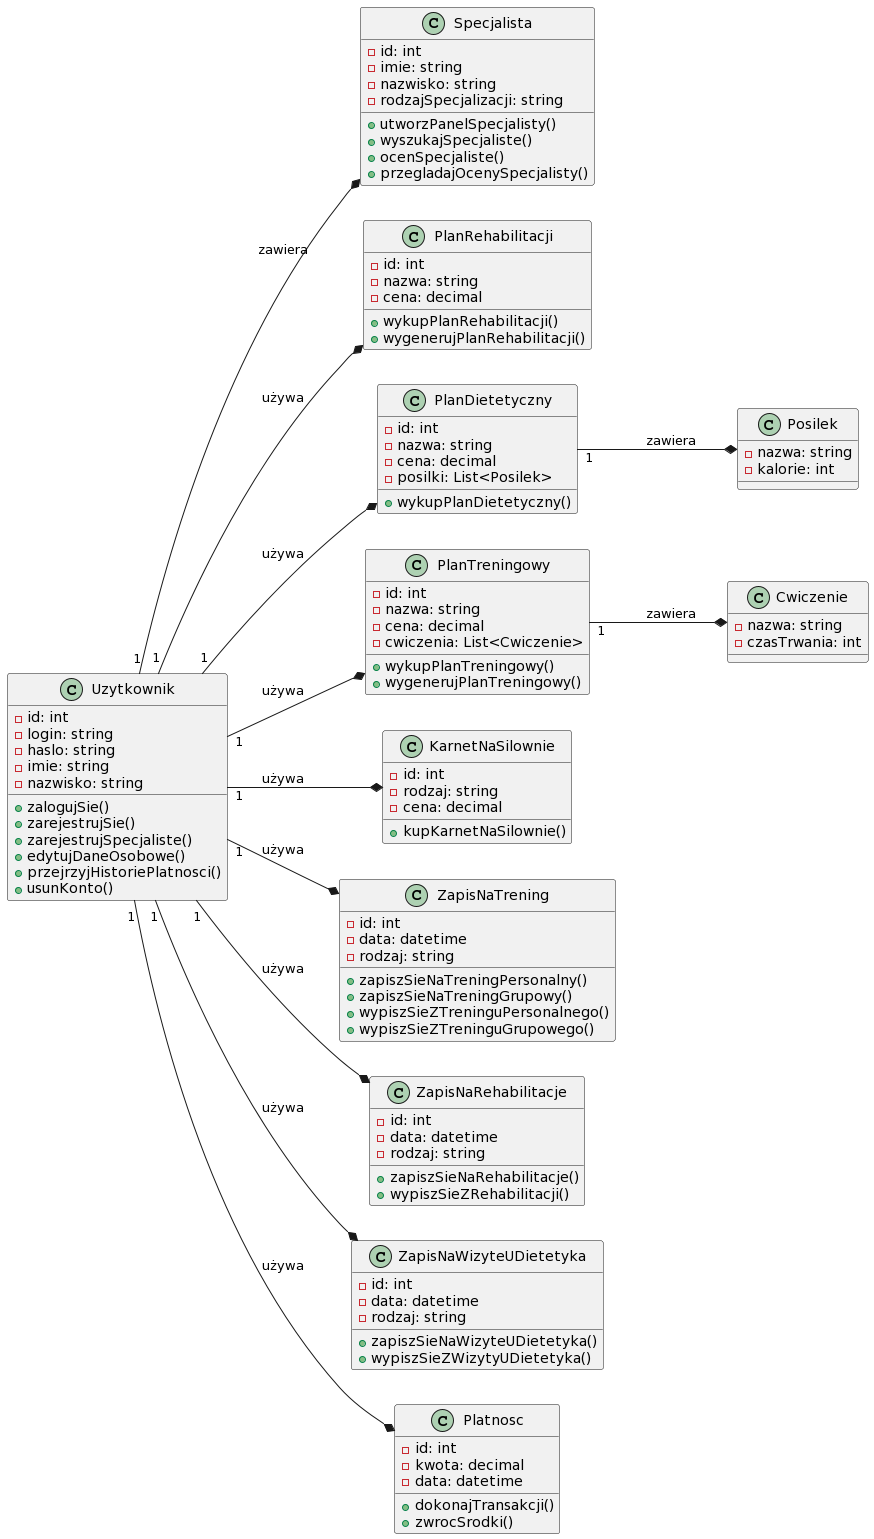
\includegraphics{../diagrams/use_cases/uzytkownik}}

{\includegraphics{../diagrams/use_cases/wypisywanie}}

{\includegraphics{../diagrams/use_cases/zapisy}}

{\includegraphics{../diagrams/use_cases/rejestracja}}

\begin{enumerate}
\setcounter{enumi}{30}
\tightlist
\item
  {Zaloguj się}
\end{enumerate}

{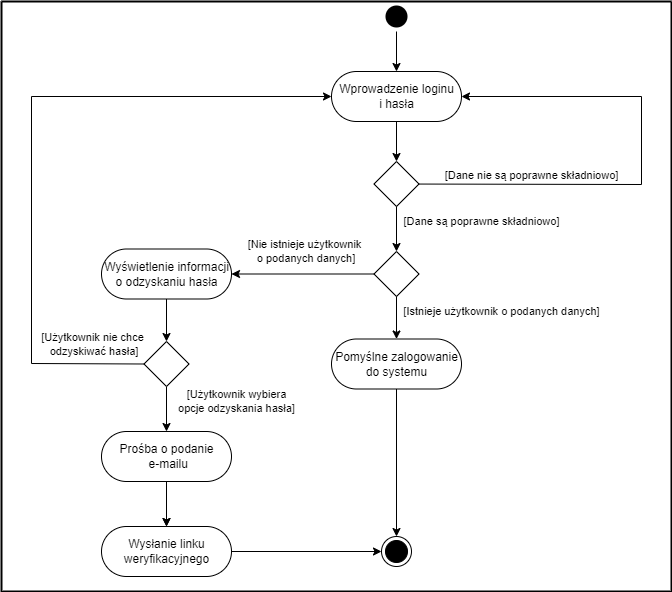
\includegraphics{../diagrams/activity/logowanie_uzytkownika_activity.png}}

{Aktorzy biorący udział: Użytkownik.}

{Cel przypadku: Umożliwienie użytkownikowi dostępu do systemu za pomocą
autoryzacji poprzez login i hasło.}

{Warunki początkowe: Użytkownik posiada poprawny login i hasło, które
zostały już utworzone. System wymaga, aby użytkownik był uwierzytelniony
przed dostępem do chronionych zasobów.}

{Warunki końcowe: Po zalogowaniu użytkownik uzyskuje dostęp do
chronionych zasobów, które zostały mu przydzielone przez system.}

{Główny ciąg zdarzeń:}

\begin{enumerate}
\tightlist
\item
  {~Użytkownik otwiera stronę logowania.}
\item
  {System wyświetla formularz logowania z polami loginu i hasła.}
\item
  {Użytkownik wprowadza swoje dane uwierzytelniające.}
\item
  {System sprawdza poprawność wprowadzonych danych uwierzytelniających.}
\item
  {System autoryzuje użytkownika i umożliwia mu dostęp do chronionych
  zasobów.}
\end{enumerate}

{~~~~~~~~Alternatywny ciąg zdarzeń:}

\begin{itemize}
\tightlist
\item
  {Jeśli wprowadzone dane uwierzytelniające są nieprawidłowe, system
  wyświetla komunikat o błędnych danych uwierzytelniających i prosi
  użytkownika o ponowne wprowadzenie poprawnych danych. Wyświetla także
  komunikat o możliwości odzyskania hasła.\\
  \strut \\
  }
\end{itemize}

\begin{enumerate}
\setcounter{enumi}{31}
\tightlist
\item
  {Zarejestruj się}
\end{enumerate}

{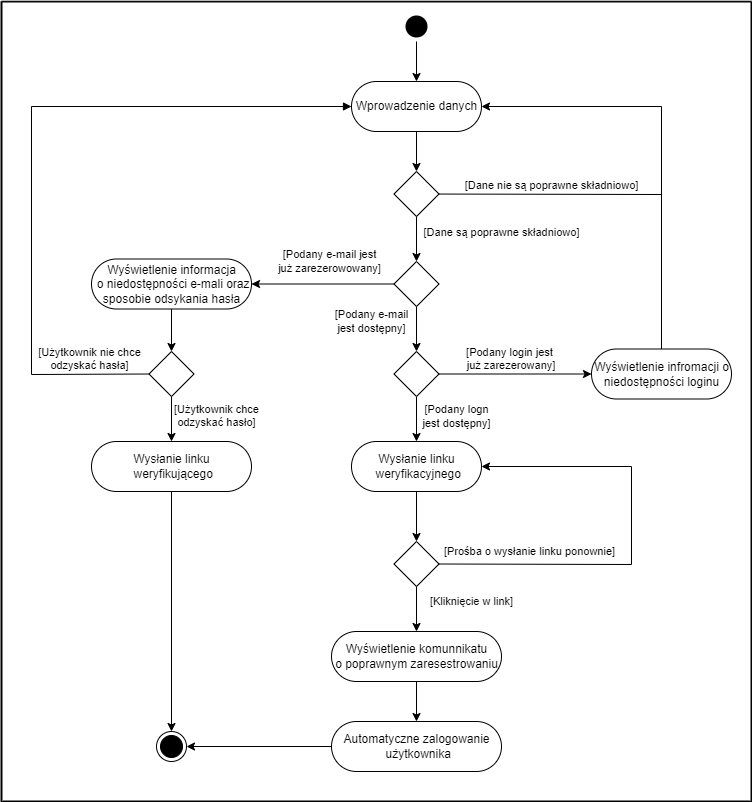
\includegraphics{../diagrams/activity/rejestracja_uzytkownika_activity.png}}

{Aktorzy biorący udział: Użytkownik.}

{Cel przypadku: ~Umożliwienie użytkownikowi utworzenia nowego konta w
systemie.}

{Warunki początkowe: Użytkownik nie ma jeszcze konta w systemie i chce
się zarejestrować.\\
Warunki końcowe: Po rejestracji użytkownik uzyskuje dostęp do systemu i
może korzystać z jego funkcjonalności.}

{Główny ciąg zdarzeń:}

\begin{enumerate}
\tightlist
\item
  {Użytkownik otwiera stronę rejestracji.}
\item
  {System wyświetla formularz rejestracyjny z polami do wprowadzenia
  danych użytkownika.}
\item
  {Użytkownik wprowadza swoje dane osobowe i dane do logowania (login i
  hasło).}
\item
  {System sprawdza poprawność wprowadzonych danych i wyświetla komunikat
  o sukcesie rejestracji.}
\item
  {Użytkownik zostaje automatycznie zalogowany do systemu i uzyskuje
  dostęp do funkcjonalności systemu.}
\end{enumerate}

{~~~~~~~~Alternatywny ciąg zdarzeń:}

\begin{itemize}
\tightlist
\item
  {Jeśli wprowadzone dane są niepoprawne, system wyświetla komunikat o
  błędzie i prosi użytkownika o poprawienie danych.}
\item
  {Jeśli login wprowadzony przez użytkownika jest już zajęty, system
  wyświetla komunikat o błędzie i prosi użytkownika o wybór innego
  loginu.}
\item
  {Użytkownik otrzymuje wiadomość e-mail z prośbą o potwierdzenie
  rejestracji klikając w link aktywacyjny, który weryfikuje poprawność
  wprowadzonych danych.}
\item
  {Jeśli użytkownik nie potwierdzi rejestracji w określonym czasie,
  system usuwa konto użytkownika i informuje go o tym.\\
  }
\end{itemize}

{}

\begin{enumerate}
\setcounter{enumi}{32}
\tightlist
\item
  {Zarejestruj specjalistę}
\end{enumerate}

{Aktorzy biorący udział: Użytkownik.}

{Cel przypadku: ~Umożliwienie użytkownikowi utworzenia nowego konta w
systemie jako specjalista.}

{Warunki początkowe: Użytkownik nie ma jeszcze konta jako specjalista w
systemie i chce się zarejestrować.\\
Warunki końcowe: Po rejestracji użytkownik uzyskuje dostęp do systemu i
może korzystać z jego rozszerzonych funkcjonalności jako specjalista.}

{Główny ciąg zdarzeń:}

\begin{enumerate}
\tightlist
\item
  {Użytkownik otwiera stronę rejestracji.}
\item
  {System wyświetla formularz rejestracyjny z polami do wprowadzenia
  danych użytkownika i dodatkowymi danymi dotyczącymi specjalizacji.}
\item
  {Użytkownik wprowadza swoje dane osobowe i dane do logowania (login i
  hasło) oraz dane potwierdzające jego specjalizacje.}
\item
  {System sprawdza poprawność wprowadzonych danych i wyświetla komunikat
  o sukcesie rejestracji.}
\item
  {Użytkownik zostaje automatycznie zalogowany do systemu jako
  specjalista i uzyskuje dostęp do rozszerzonych funkcjonalności
  systemu.}
\end{enumerate}

{~~~~~~~~Alternatywny ciąg zdarzeń:}

\begin{itemize}
\tightlist
\item
  {Jeśli wprowadzone dane są niepoprawne, system wyświetla komunikat o
  błędzie i prosi użytkownika o poprawienie danych.}
\item
  {Jeśli login wprowadzony przez użytkownika jest już zajęty, system
  wyświetla komunikat o błędzie i prosi użytkownika o wybór innego
  loginu.}
\item
  {Użytkownik otrzymuje wiadomość e-mail z prośbą o potwierdzenie
  rejestracji klikając w link aktywacyjny, który weryfikuje poprawność
  wprowadzonych danych.}
\item
  {Jeśli użytkownik nie potwierdzi rejestracji w określonym czasie,
  system usuwa konto użytkownika i informuje go o tym.\\
  \strut \\
  }
\end{itemize}

\begin{enumerate}
\setcounter{enumi}{33}
\tightlist
\item
  {Stwórz panel specjalisty
  \textless\textless extend\textgreater\textgreater{}}
\end{enumerate}

{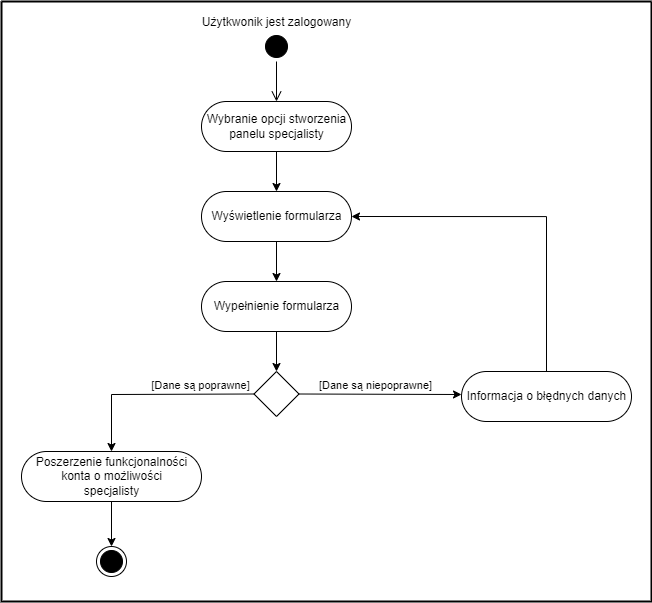
\includegraphics{../diagrams/activity/stworzenie_panelu_specjalisty_activity.png}}

{Aktorzy biorący udział: Użytkownik.}

{Cel przypadku: ~Umożliwienie użytkownikowi utworzenia panelu
specjalisty, który umożliwi mu zarządzanie zasobami i danymi w systemie
dostarczając dodatkowych funkcjonalności.}

{Warunki początkowe: Użytkownik posiada konto w systemie i jest
zalogowany. System umożliwia tworzenie panelu dla specjalisty.\\
Warunki końcowe: Po stworzeniu panelu specjalista użytkownik uzyskuje
dostęp do zasobów i danych, które umożliwią mu pracę jako specjalista.}

{Główny ciąg zdarzeń:}

\begin{enumerate}
\tightlist
\item
  {Użytkownik loguje się do systemu i otwiera stronę tworzenia panelu
  specjalisty.}
\item
  {System wyświetla formularz tworzenia panelu, w którym użytkownik
  wprowadza dane potwierdzające specjalizację.}
\item
  {System tworzy nowy panel i przypisuje go do konta użytkownika jako
  panel specjalisty.}
\item
  {Użytkownik zostaje poinformowany o utworzeniu nowego panelu i
  uzyskuje dostęp do zasobów i danych, które umożliwią mu zarządzanie
  swoją pracą w systemie jako specjalista.}
\end{enumerate}

{~~~~~~~~Alternatywny ciąg zdarzeń:}

\begin{itemize}
\tightlist
\item
  {Jeśli system napotka problem podczas tworzenia panelu, wyświetla
  komunikat o błędzie i informuje użytkownika o tym. Użytkownik może
  spróbować stworzyć panel ponownie lub skontaktować się z działem
  obsługi technicznej w celu rozwiązania problemu.\\
  \strut \\
  }
\end{itemize}

\begin{enumerate}
\setcounter{enumi}{34}
\tightlist
\item
  {Wykup plan rehabilitacji
  \textless\textless include\textgreater\textgreater{}}
\end{enumerate}

{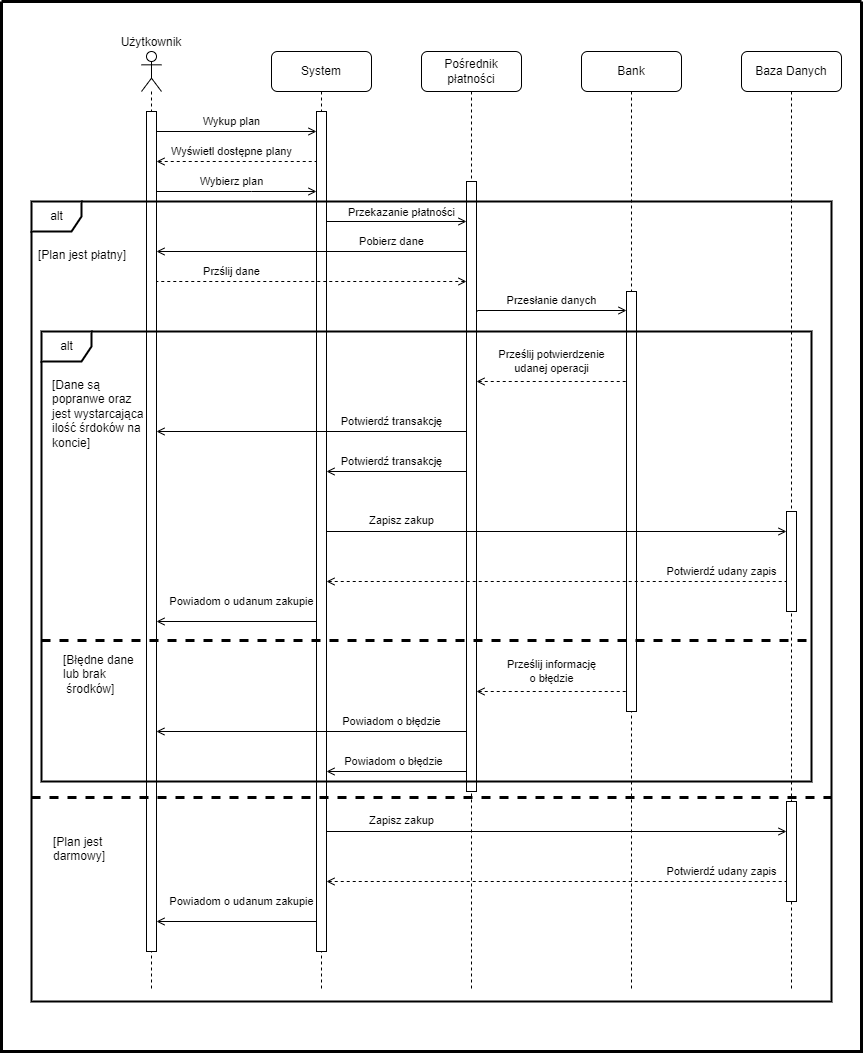
\includegraphics{../diagrams/sequence/wykupienie_planu_sequence.png}}

{Aktorzy biorący udział: Użytkownik.}

{Cel przypadku: ~Umożliwienie użytkownikowi dokonania płatności i
uzyskania dostępu do specjalistycznych programów rehabilitacyjnych w
systemie.}

{Warunki początkowe: Użytkownik posiada konto w systemie i jest
zalogowany. System umożliwia wykupienie planu rehabilitacji.\\
Warunki końcowe: Użytkownik dokonuje płatności i uzyskuje dostęp do
specjalistycznych programów rehabilitacyjnych w systemie.}

{Główny ciąg zdarzeń:}

\begin{enumerate}
\tightlist
\item
  {Użytkownik loguje się do systemu i otwiera stronę wykupu planu
  rehabilitacji.}
\item
  {System wyświetla listę dostępnych planów rehabilitacyjnych wraz z ich
  opisem i cenami.}
\item
  {Użytkownik wybiera plan rehabilitacyjny, który chce wykupić i klika
  przycisk "Kup teraz".}
\item
  {System wyświetla formularz płatności, w którym użytkownik może
  wprowadzić swoje dane oraz informacje o karcie kredytowej lub innym
  sposobie płatności.}
\item
  {Użytkownik wprowadza swoje dane oraz informacje o płatności i kliknie
  przycisk "Zapłać".}
\item
  {System przetwarza płatność i udziela użytkownikowi dostępu do planu
  rehabilitacyjnego.}
\end{enumerate}

{~~~~~~~~Alternatywny ciąg zdarzeń:}

\begin{itemize}
\tightlist
\item
  {Jeśli system wykryje błąd w informacjach o płatności lub karcie
  kredytowej, wyświetla komunikat o błędzie i prosi użytkownika o
  poprawienie informacji.}
\item
  {Jeśli płatność nie zostanie zaakceptowana, system wyświetla
  informacje o nieudanej płatności i prosi użytkownika o wybranie innego
  sposobu płatności lub skontaktowanie się z działem obsługi
  technicznej.}
\item
  {Jeśli rehabilitacja jest darmowa użytkownik jedynie wprowadza swoje
  dane.}
\end{itemize}

{\hfill\break
}

\begin{enumerate}
\setcounter{enumi}{35}
\tightlist
\item
  {Wykup plan dietetyczny}
\end{enumerate}

{Aktorzy biorący udział: Użytkownik.}

{Cel przypadku: ~Umożliwienie użytkownikowi dokonania płatności i
uzyskania dostępu do indywidualnie dopasowanych planów żywieniowych i
porad dietetycznych.}

{Warunki początkowe: Użytkownik posiada konto w systemie i jest
zalogowany. System umożliwia wykupienie planu dietetycznego.\\
Warunki końcowe: Użytkownik dokonuje płatności i uzyskuje dostęp do
indywidualnie dopasowanych planów żywieniowych i porad dietetycznych w
systemie.}

{Główny ciąg zdarzeń:}

\begin{enumerate}
\tightlist
\item
  {Użytkownik loguje się do systemu i otwiera stronę wykupu planu
  dietetycznego.}
\item
  {System wyświetla listę dostępnych planów dietetycznych wraz z ich
  opisem i cenami.}
\item
  {Użytkownik wybiera plan dietetyczny, który chce wykupić i klika
  przycisk "Kup teraz".}
\item
  {System wyświetla formularz płatności, w którym użytkownik może
  wprowadzić swoje dane oraz informacje o karcie kredytowej lub innym
  sposobie płatności.}
\item
  {Użytkownik wprowadza swoje dane oraz informacje o płatności i kliknie
  przycisk "Zapłać".}
\item
  {System przetwarza płatność i udziela użytkownikowi dostępu do
  indywidualnie dopasowanych planów żywieniowych i porad dietetycznych.}
\end{enumerate}

{~~~~~~~~Alternatywny ciąg zdarzeń:}

\begin{itemize}
\tightlist
\item
  {Jeśli system wykryje błąd w informacjach o płatności lub karcie
  kredytowej, wyświetla komunikat o błędzie i prosi użytkownika o
  poprawienie informacji.}
\item
  {Jeśli płatność nie zostanie zaakceptowana, system wyświetla
  informacje o nieudanej płatności i prosi użytkownika o wybranie innego
  sposobu płatności lub skontaktowanie się z działem obsługi
  technicznej.}
\item
  {Jeśli plan dietetyczny jest darmowy użytkownik jedynie wprowadza
  swoje dane.}
\end{itemize}

{\hfill\break
}

\begin{enumerate}
\setcounter{enumi}{36}
\tightlist
\item
  {Wykup plan treningowy}
\end{enumerate}

{Aktorzy biorący udział: Użytkownik.}

{Cel przypadku: ~Umożliwienie użytkownikowi wykupienia planu
treningowego, który zostanie dostarczony przez platformę.}

{Warunki początkowe: Użytkownik musi być zalogowany na swoim koncie.\\
Warunki końcowe: Użytkownik wykupuje plan treningowy, który jest
aktualnie dostępny. Użytkownik otrzymuje potwierdzenie zakupu i plan
treningowy dostępny w jego panelu.}

{Główny ciąg zdarzeń:}

\begin{enumerate}
\tightlist
\item
  {Użytkownik wybiera z menu opcję "Wykup plan treningowy".}
\item
  {System wyświetla listę dostępnych planów treningowych wraz z cenami i
  opisami.}
\item
  {Użytkownik wybiera plan treningowy, który chce wykupić.}
\item
  {System wyświetla podsumowanie wybranego planu treningowego oraz
  informacje dotyczące płatności.}
\item
  {Użytkownik dokonuje płatności za plan treningowy.}
\item
  {System potwierdza dokonanie płatności i udostępnia użytkownikowi
  dostęp do planu treningowego w panelu użytkownika.}
\end{enumerate}

{~~~~~~~~Alternatywny ciąg zdarzeń:}

\begin{itemize}
\tightlist
\item
  {W przypadku niepowodzenia płatności, system informuje użytkownika o
  błędzie i proponuje powtórzenie transakcji lub wybór innej metody
  płatności.}
\item
  {Jeśli plan treningowy jest darmowy użytkownik jedynie wprowadza swoje
  dane.\\
  }
\end{itemize}

{}

\begin{enumerate}
\setcounter{enumi}{37}
\tightlist
\item
  {Kup karnet na siłownię}
\end{enumerate}

{Aktorzy biorący udział: Użytkownik.}

{Cel przypadku: Umożliwienie użytkownikowi zakupu karnetu na siłownię,
który pozwoli mu na korzystanie z usług siłowni przez określony czas.}

{Warunki początkowe: Użytkownik musi być zalogowany na swoim koncie.\\
Warunki końcowe: Użytkownik wykupuje plan treningowy, który jest
dostępny w panelu użytkownika. Użytkownik otrzymuje potwierdzenie zakupu
i plan treningowy dostępny w jego panelu.}

{Główny ciąg zdarzeń:}

\begin{enumerate}
\tightlist
\item
  {Użytkownik wybiera z menu opcję "Kup karnet na siłownię".}
\item
  {System wyświetla listę dostępnych karnetów wraz z cenami i opisami.}
\item
  {Użytkownik wybiera karnet, który chce kupić.}
\item
  {System wyświetla podsumowanie wybranego karnetu oraz informacje
  dotyczące płatności.}
\item
  {Użytkownik dokonuje płatności za karnet.}
\item
  {System potwierdza dokonanie płatności i udostępnia użytkownikowi
  informacje dotyczące karnetu w panelu użytkownika.}
\end{enumerate}

{~~~~~~~~Alternatywny ciąg zdarzeń:}

\begin{itemize}
\tightlist
\item
  {W przypadku niepowodzenia płatności, system informuje użytkownika o
  błędzie i proponuje powtórzenie transakcji lub wybór innej metody
  płatności.\\
  \strut \\
  }
\end{itemize}

\begin{enumerate}
\setcounter{enumi}{38}
\tightlist
\item
  {Zapisz się na trening personalny}
\end{enumerate}

{Aktorzy biorący udział: Użytkownik.}

{Cel przypadku: umożliwienie użytkownikowi zapisu na trening personalny
z trenerem siłowni.}

{Warunki początkowe: Użytkownik musi być zalogowany na swoje konto.}

{Musi być dostępna wolna godzina treningowa z wybranym trenerem.}

{Warunki końcowe: Użytkownik zostaje zapisany na trening personalny z
wybranym trenerem. System wyświetla potwierdzenie zapisu.}

{Główny ciąg zdarzeń:}

\begin{enumerate}
\tightlist
\item
  {Użytkownik wybiera z menu opcję "Zapisz się na trening personalny".}
\item
  {System wyświetla listę dostępnych trenerów oraz wolne godziny
  treningowe.}
\item
  {Użytkownik wybiera trenera oraz godzinę treningową, na którą chce się
  zapisać.}
\item
  {System wyświetla podsumowanie wyboru oraz informacje o cenie
  treningu.}
\item
  {Użytkownik potwierdza zapis na trening personalny dokonując
  płatności.}
\item
  {System wyświetla potwierdzenie zapisu i informacje o treningu.}
\end{enumerate}

{~~~~~~~~Alternatywny ciąg zdarzeń:}

\begin{itemize}
\tightlist
\item
  {Jeśli nie ma wolnej godziny z wybranym trenerem, system informuje
  użytkownika o braku dostępności i proponuje wybór innego trenera lub
  godziny.}
\item
  {W przypadku braku potwierdzenia zapisu przez użytkownika, system
  anuluje proces zapisu na trening personalny.}
\item
  {Jeśli z pewnych przyczyn trening nie będzie mógł się odbyć użytkownik
  zostanie poproszony o wybranie nowego terminu lub otrzyma zwrot
  kosztów za zapis.}
\item
  {W przypadku, gdy trening personalny jest darmowy użytkownik jedynie
  będzie musiał wprowadzić swoje dane}
\item
  {W przypadku niepowodzenia płatności, system informuje użytkownika o
  błędzie i proponuje powtórzenie transakcji lub wybór innej metody
  płatności.\\
  \strut \\
  \strut \\
  }
\end{itemize}

\begin{enumerate}
\setcounter{enumi}{39}
\tightlist
\item
  {Zapisz się na rehabilitację}
\end{enumerate}

{Aktorzy biorący udział: Użytkownik.}

{Cel przypadku: Umożliwienie użytkownikowi zapisu na rehabilitację}

{Warunki początkowe: Użytkownik musi być zalogowany na swoje konto.
Muszą być dostępne wolne terminy na rehabilitację.}

{Warunki końcowe: Użytkownik zostaje zapisany na wybraną rehabilitację.
System wyświetla potwierdzenie zapisu.}

{Główny ciąg zdarzeń:}

\begin{enumerate}
\tightlist
\item
  {Użytkownik wybiera z menu opcję "Zapisz się na rehabilitację".}
\item
  {System wyświetla listę dostępnych rehabilitacji oraz wolne terminy.}
\item
  {Użytkownik wybiera rehabilitację na który chce się zapisać oraz jej
  termin.}
\item
  {System wyświetla podsumowanie wyboru oraz informacje o cenie
  rehabilitacji.}
\item
  {Użytkownik potwierdza zapis na rehabilitację.}
\item
  {System wyświetla potwierdzenie zapisu i informacje o rehabilitacji.}
\end{enumerate}

{~~~~~~~~Alternatywny ciąg zdarzeń:}

\begin{itemize}
\tightlist
\item
  {Jeśli nie ma wolnego terminu w wybranej placówce, system informuje
  użytkownika o braku dostępności i proponuje wybór innej placówki lub
  terminu.}
\item
  {W przypadku braku potwierdzenia zapisu przez użytkownika, system
  anuluje proces zapisu na rehabilitację.}
\item
  {W przypadku niepowodzenia płatności, system informuje użytkownika o
  błędzie i proponuje powtórzenie transakcji lub wybór innej metody
  płatności.}
\item
  {Jeśli rehabilitacja jest darmowa użytkownik zostanie poproszony
  jedynie o podanie swoich danych osobowych.}
\end{itemize}

{\hfill\break
}

\begin{enumerate}
\setcounter{enumi}{40}
\tightlist
\item
  {Zapisz się na wizytę u dietetyka}
\end{enumerate}

{Aktorzy biorący udział: Użytkownik.}

{Cel przypadku: Zapisanie się na wizytę u dietetyka w celu uzyskania
porady i pomocy w zakresie odżywiania.}

{Warunki początkowe: Użytkownik jest zalogowany w systemie.}

{W systemie istnieją wolne terminy dla dietetyka.}

{Warunki końcowe: Użytkownik zostaje zapisany na wizytę u dietetyka w
wybranym terminie. System pobiera opłatę za wizytę z konta użytkownika.}

{Główny ciąg zdarzeń:}

\begin{enumerate}
\tightlist
\item
  {Użytkownik wybiera opcję "Zapisz się na wizytę u dietetyka" w menu.}
\item
  {System wyświetla dostępne terminy u dietetyka.}
\item
  {Użytkownik wybiera dogodny dla siebie termin wizyty.}
\item
  {System wyświetla podsumowanie wizyty, w tym jej cenę.}
\item
  {Użytkownik potwierdza wizytę i opłaca ją z konta.}
\item
  {System zapisuje wizytę użytkownika i wysyła mu potwierdzenie.}
\end{enumerate}

{~~~~~~~~Alternatywny ciąg zdarzeń:}

\begin{itemize}
\tightlist
\item
  {W przypadku braku wolnych terminów system informuje użytkownika o tym
  i proponuje wybór innego terminu.}
\item
  {W przypadku braku wystarczającej ilości środków na koncie, system
  prosi użytkownika o doładowanie konta lub wybór innej formy
  płatności.}
\end{itemize}

{\hfill\break
}

\begin{enumerate}
\setcounter{enumi}{41}
\tightlist
\item
  {Zapisz się na trening grupowy}
\end{enumerate}

{Aktorzy biorący udział: Użytkownik.}

{Cel przypadku: Zapisanie się użytkownika na trening grupowy w wybranym
terminie.}

{Warunki początkowe: Użytkownik jest zalogowany do swojego konta.
Użytkownik ma dostęp do kalendarza treningów grupowych. W systemie
istnieją dostępne treningi grupowe z wolnymi miejscami.}

{Warunki końcowe: Użytkownik zostaje zapisany na wybrany przez siebie
trening grupowy. W systemie odnotowana jest informacja o zapisie
użytkownika na trening.}

{Główny ciąg zdarzeń:}

\begin{enumerate}
\tightlist
\item
  {Użytkownik wybiera opcję "Zapisz się na trening grupowy".}
\item
  {System wyświetla kalendarz z dostępnymi terminami treningów
  grupowych.}
\item
  {Użytkownik wybiera wybrany termin treningu.}
\item
  {System wyświetla szczegóły treningu (np. nazwa, prowadzący, czas
  trwania).}
\item
  {Użytkownik potwierdza wybór treningu dokonując płatności za trening.}
\item
  {System zapisuje użytkownika na trening grupowy.}
\end{enumerate}

{~~~~~~~~Alternatywny ciąg zdarzeń:}

\begin{itemize}
\tightlist
\item
  {Jeśli w wybranym terminie nie ma wolnych miejsc na treningu grupowym,
  system wyświetla informację o braku miejsc i proponuje wybór innego
  terminu.}
\item
  {Użytkownik ma możliwość anulowania zapisu na trening grupowy przed
  rozpoczęciem treningu. W takim przypadku system usuwa informację o
  zapisie użytkownika na trening. W przypadku anulowania zapisu
  przynajmniej tydzień przed rozpoczęciem treningu środki na konto za
  trening zostają zwrócone na konto użytkownika.}
\item
  {W przypadku braku wystarczającej ilości środków na koncie, system
  prosi użytkownika o doładowanie konta lub wybór innej formy
  płatności.}
\item
  {Jeśli trening grupowy jest darmowy użytkownik jest proszony jedynie o
  wprowadzenie swoich danych osobowych.\\
  }
\end{itemize}

{}

\begin{enumerate}
\setcounter{enumi}{42}
\tightlist
\item
  {Wypisz się z treningu personalnego}
\end{enumerate}

{Aktorzy biorący udział: Użytkownik.}

{Cel przypadku: Wypisanie się użytkownika z treningu personalnego.}

{Warunki początkowe: Użytkownik musi być zalogowany i zapisany na
trening personalny. }

{Warunki końcowe: Trening zostaje odwołany. Trener personalny dostaje
informację poprzez aplikację. Jeśli trening został opłacony zostają
zwrócone środki lub ich część.}

{Główny ciąg zdarzeń: }

\begin{enumerate}
\tightlist
\item
  {Użytkownik wchodzi w panel nadchodzących spotkań.}
\item
  {Użytkownik wybiera interesujący go trening.}
\item
  {Użytkownik klika przycisk ``usuń''.}
\end{enumerate}

{~~~~~~~~Alternatywny ciąg zdarzeń:}

\begin{itemize}
\tightlist
\item
  {Jeśli trening z innych przyczyn nie jest już dostępny użytkownik
  dostaję informację, że dany trening jest już usunięty.}
\item
  {W przypadku błędu ze strony pośrednika płatności użytkownik zostaje o
  nim poinformowany. Użytkownik może następnie ponowić zwrot środków.}
\item
  {Jeśli trening został opłacony z zaliczką, zaliczka nie jest
  zwracana.}
\end{itemize}

{}

\begin{enumerate}
\setcounter{enumi}{43}
\tightlist
\item
  {Wypisz się z rehabilitacji}
\end{enumerate}

{Aktorzy biorący udział: Użytkownik.}

{Cel przypadku: Wypisanie się użytkownika z sesji rehabilitacyjnej.}

{Warunki początkowe: Użytkownik musi być zalogowany i zapisany na sesję
rehabilitacyjną. }

{Warunki końcowe: Sesja rehabilitacyjna zostaje odwołana. Fizjoterapeuta
dostaje informację poprzez aplikację. Jeśli sesja rehabilitacyjna
została opłacona zostają zwrócone środki lub ich część.}

{Główny ciąg zdarzeń: }

\begin{enumerate}
\tightlist
\item
  {Użytkownik wchodzi w panel nadchodzących spotkań.}
\item
  {Użytkownik wybiera interesującą go sesję.}
\item
  {Użytkownik klika przycisk ``usuń''.}
\end{enumerate}

{~~~~~~~~Alternatywny ciąg zdarzeń:}

\begin{itemize}
\tightlist
\item
  {Jeśli sesja z innych przyczyn nie jest już dostępna użytkownik
  dostaję informację, że dana sesja jest już usunięta.}
\item
  {W przypadku błędu ze strony pośrednika płatności użytkownik zostaje o
  nim poinformowany. Użytkownik może następnie ponowić zwrot środków.}
\item
  {Jeśli sesja została opłacona z zaliczką, zaliczka nie jest zwracana.}
\end{itemize}

{}

\begin{enumerate}
\setcounter{enumi}{44}
\tightlist
\item
  {Wypisz się z wizyty u dietetyka}
\end{enumerate}

{Aktorzy biorący udział: Użytkownik.}

{Cel przypadku: Wypisanie się użytkownika z wizyty.}

{Warunki początkowe: Użytkownik musi być zalogowany i zapisany na
wizytę. }

{Warunki końcowe: Wizyta zostaje odwołana. Dietetyk dostaje informację
poprzez aplikację. Jeśli wizyta została opłacona zostają zwrócone środki
lub ich część.}

{Główny ciąg zdarzeń: }

\begin{enumerate}
\tightlist
\item
  {Użytkownik wchodzi w panel nadchodzących spotkań.}
\item
  {Użytkownik wybiera interesującą go wizytę.}
\item
  {Użytkownik klika przycisk ``usuń''.}
\end{enumerate}

{~~~~~~~~Alternatywny ciąg zdarzeń:}

\begin{itemize}
\tightlist
\item
  {Jeśli wizyta z innych przyczyn nie jest już dostępna użytkownik
  dostaję informację, że dana wizyta jest już usunięta.}
\item
  {W przypadku błędu ze strony pośrednika płatności użytkownik zostaje o
  nim poinformowany. Użytkownik może następnie ponowić zwrot środków.}
\item
  {Jeśli sesja została opłacona z zaliczką, zaliczka nie jest zwracana.}
\end{itemize}

{}

\begin{enumerate}
\setcounter{enumi}{45}
\tightlist
\item
  {Wypisz się z treningu grupowego}
\end{enumerate}

{Aktorzy biorący udział: Użytkownik.}

{Cel przypadku: Wypisanie się użytkownika z treningu grupowego.}

{Warunki początkowe: Użytkownik musi być zalogowany i zapisany na
trening grupowy. }

{Warunki końcowe: Użytkownik jest wypisany z treningu. Jeśli trening
został opłacony zostają zwrócone środki lub ich część.}

{Główny ciąg zdarzeń: }

\begin{enumerate}
\tightlist
\item
  {Użytkownik wchodzi w panel nadchodzących spotkań.}
\item
  {Użytkownik wybiera interesujący go trening.}
\item
  {Użytkownik klika przycisk ``usuń''.}
\end{enumerate}

{~~~~~~~~Alternatywny ciąg zdarzeń:}

\begin{itemize}
\tightlist
\item
  {Jeśli trening z innych przyczyn nie jest już dostępny użytkownik
  dostaję informację, że dany trening jest już usunięty.}
\item
  {W przypadku błędu ze strony pośrednika płatności użytkownik zostaje o
  nim poinformowany. Użytkownik może następnie ponowić zwrot środków.}
\item
  {Jeśli trening został opłacony z zaliczką, zaliczka nie jest
  zwracana.}
\end{itemize}

{}

\begin{enumerate}
\setcounter{enumi}{46}
\tightlist
\item
  {Wygeneruj plan treningowy}
\end{enumerate}

{Aktorzy biorący udział: Użytkownik.}

{Cel przypadku: Użytkownik dostaje gotowy plan treningu wygenerowany
przez system.}

{Warunki początkowe: -}

{Warunki końcowe: Użytkownik ma zapisany plan treningowy, który został
wygenerowany.}

{Główny ciąg zdarzeń:}

\begin{enumerate}
\tightlist
\item
  {Użytkownik wchodzi w sekcję ``moje plany''.}
\item
  {Użytkownik klika przycisk ``wygeneruj plan''.}
\item
  {Użytkownik podaje potrzebne informacje w formularzu.}
\item
  {Użytkownik dostaje gotowy plan do swojej sekcji ``moje plany''.}
\end{enumerate}

{}

\begin{enumerate}
\setcounter{enumi}{47}
\tightlist
\item
  {Wygeneruj plan rehabilitacji}
\end{enumerate}

{Aktorzy biorący udział: Użytkownik.}

{Cel przypadku: Użytkownik dostaje gotowy plan rehabilitacji
wygenerowany przez system.}

{Warunki początkowe: -}

{Warunki końcowe: Użytkownik ma zapisany plan rehabilitacji, który
został wygenerowany.}

{Główny ciąg zdarzeń:}

\begin{enumerate}
\tightlist
\item
  {Użytkownik wchodzi w sekcję ``moje plany''.}
\item
  {Użytkownik klika przycisk ``wygeneruj plan''.}
\item
  {Użytkownik podaje potrzebne informacje w formularzu.}
\item
  {Użytkownik dostaje gotowy plan do swojej sekcji ``moje plany''.}
\end{enumerate}

{}

\begin{enumerate}
\setcounter{enumi}{48}
\tightlist
\item
  {Wyszukaj specjalistę}
\end{enumerate}

{Aktorzy biorący udział: Użytkownik.}

{Cel przypadku: Wyświetlenie użytkownikowi dostępnych specjalistów.}

{Warunki początkowe: -}

{Warunki końcowe: Użytkownik widzi listę dostępnych specjalistów.}

{Główny ciąg zdarzeń:}

\begin{enumerate}
\tightlist
\item
  {Użytkownik wchodzi w sekcję ``specjaliści''.}
\item
  {Użytkownik wyszukuję dany typ specjalisty.}
\item
  {Użytkownik widzi rezultat wyszukiwania.}
\end{enumerate}

{}

\begin{enumerate}
\setcounter{enumi}{49}
\tightlist
\item
  {Oceń specjalistę}
\end{enumerate}

{Aktorzy biorący udział: Użytkownik.}

{Cel przypadku: Użytkownik wystawia subiektywną ocenę dla danego
specjalisty.}

{Warunki początkowe: Użytkownik jest zalogowany.}

{Warunki końcowe: Ocena użytkownika zostaje dodana.}

{Główny ciąg zdarzeń:}

\begin{enumerate}
\tightlist
\item
  {Użytkownik wchodzi w sekcję ``specjaliści''.}
\item
  {Użytkownik wyszukuję konkretnego specjalistę.}
\item
  {Użytkownik wystawia ocenę i opis swoich odczuć co do obsługi.}
\end{enumerate}

{}

\begin{enumerate}
\setcounter{enumi}{50}
\tightlist
\item
  {Przeglądaj oceny specjalisty}
\end{enumerate}

{Aktorzy biorący udział: Użytkownik.}

{Cel przypadku: Wyświetlenie użytkownikowi ocen dla danego specjalisty.}

{Warunki początkowe: -}

{Warunki końcowe: Użytkownik widzi oceny dla danego specjalisty..}

{Główny ciąg zdarzeń:}

\begin{enumerate}
\tightlist
\item
  {Użytkownik wchodzi w sekcję ``specjaliści''.}
\item
  {Użytkownik wyszukuję konkretnego specjalistę.}
\item
  {Użytkownik widzi rezultat wyszukiwania: imię, nazwisko, stanowisko,
  dostępne lokacje, średnią ocen w skali 1-5 i poszczególne oceny..}
\end{enumerate}

{}

\begin{enumerate}
\setcounter{enumi}{51}
\tightlist
\item
  {Edytuj dane osobowe}
\end{enumerate}

{Aktorzy biorący udział: Użytkownik.}

{Cel przypadku: Zmiana danych osobowych użytkownika.}

{Warunki początkowe: Użytkownik jest zalogowany.}

{Warunki końcowe: Użytkownik ma zmienione dane w systemie.}

{Główny ciąg zdarzeń:}

\begin{enumerate}
\tightlist
\item
  {Użytkownik wchodzi w sekcję ``ja''.}
\item
  {Użytkownik zmienia dane w polach, które go interesują.}
\item
  {Użytkownik klika ``potwierdź''.}
\end{enumerate}

{}

\begin{enumerate}
\setcounter{enumi}{52}
\tightlist
\item
  {Przejrzyj historię płatności}
\end{enumerate}

{Aktorzy biorący udział: Użytkownik.}

{Cel przypadku: Przejrzenie historii płatności użytkownika}

{Warunki początkowe: Użytkownik jest zalogowany.}

{Warunki końcowe: Użytkownik widzi swoją historię płatności.}

{Główny ciąg zdarzeń:}

\begin{enumerate}
\tightlist
\item
  {Użytkownik wchodzi w sekcję ``ja''.}
\item
  {System wyświetla szczegółową historię płatności użytkownika, w tym
  daty, kwoty oraz rodzaj płatności.}
\item
  {Użytkownik może przeglądać historię płatności, a także eksportować ją
  do pliku CSV lub PDF.}
\end{enumerate}

{}

\begin{enumerate}
\setcounter{enumi}{53}
\tightlist
\item
  {Usuń konto}
\end{enumerate}

{Aktorzy biorący udział: Użytkownik.}

{Cel przypadku: Usunięcie konta użytkownika.}

{Warunki początkowe: Użytkownik jest zalogowany.}

{Warunki końcowe: Konto użytkownika zostaje usunięte, lecz informacje o
płatnościach i karnetach zostają zachowane.}

{Główny ciąg zdarzeń:}

\begin{enumerate}
\tightlist
\item
  {Użytkownik wchodzi w sekcję ``ja''.}
\item
  {Użytkownik klika ``usuń konto''.}
\item
  {Użytkownik klika ``potwierdź''.}
\end{enumerate}

\includegraphics{../diagrams/use_cases/posrednik_platnosci}

